% ------------------------------------------------------------------------------
% TYPO3 CMS 8.4 - What's New - Chapter "Backend User Interface" (Serbian Version)
%
% @author	Michael Schams <schams.net>
% @license	Creative Commons BY-NC-SA 3.0
% @link		http://typo3.org/download/release-notes/whats-new/
% @language	English
% ------------------------------------------------------------------------------
% LTXE-CHAPTER-UID:		07b25346-95b1df21-a6ebe09a-49f53f41
% LTXE-CHAPTER-NAME:	Backend User Interface
% ------------------------------------------------------------------------------

\section{Backend User Interface}
\begin{frame}[fragile]
	\frametitle{Backend User Interface}

	\begin{center}\huge{Chapter 1:}\end{center}
	\begin{center}\huge{\color{typo3darkgrey}\textbf{Backend User Interface}}\end{center}

\end{frame}

% ------------------------------------------------------------------------------
% LTXE-SLIDE-START
% LTXE-SLIDE-UID:		24582de5-101c59ec-a22ea3df-dce5bb2f
% LTXE-SLIDE-ORIGIN:	75977160-b74e3317-0f697728-71b501d1 English
% LTXE-SLIDE-TITLE:		Mobile Responsive TYPO3 Backend
% ------------------------------------------------------------------------------

\begin{frame}[fragile]
	\frametitle{Backend User Interface}
	\framesubtitle{Mobile Responsive TYPO3 Backend}

	The TYPO3 Backend is fully mobile responsive now.

	\begin{figure}
		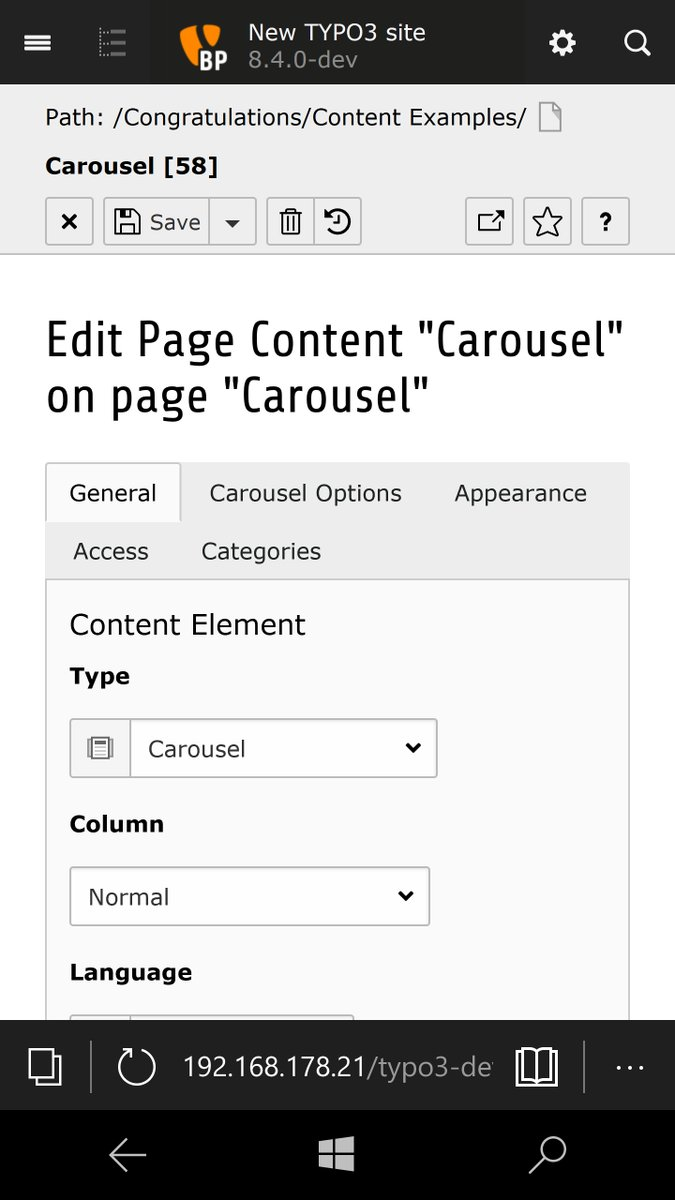
\includegraphics[width=0.25\linewidth]{BackendUserInterface/mobile-responsive-backend.jpg}
	\end{figure}

\end{frame}

% ------------------------------------------------------------------------------
% LTXE-SLIDE-START
% LTXE-SLIDE-UID:		7803115c-3a4c1594-9c819442-26f4e97c
% LTXE-SLIDE-ORIGIN:	f6668b2d-8932a470-5b9c024c-e4e9f53a English
% LTXE-SLIDE-TITLE:		Install Tool: Upgrade Analysis
% ------------------------------------------------------------------------------

\begin{frame}[fragile]
	\frametitle{Backend User Interface}
	\framesubtitle{Install Tool: Upgrade Analysis}

% The install tool, which is also a heavily used feature during updates between
% TYPO3 versions, has received some more beauty, basically finding all documented
% changes with a cool filter to show what is relevant for an integrator,
% extension author or site owner. Although this is already pretty cool, stay
% tuned for even better features to make migrations even easier between TYPO3
% versions!
% The migration and deprecation of existing options and switching within the TCA
% definitions we have in place since TYPO3 v7, is also visible in the Install Tool
% now.

	TYPO3 version upgrades made easy with the new \textbf{Upgrade Analysis} tool
	in the Install Tool (find/filter documented changes between versions).

	\begin{figure}
		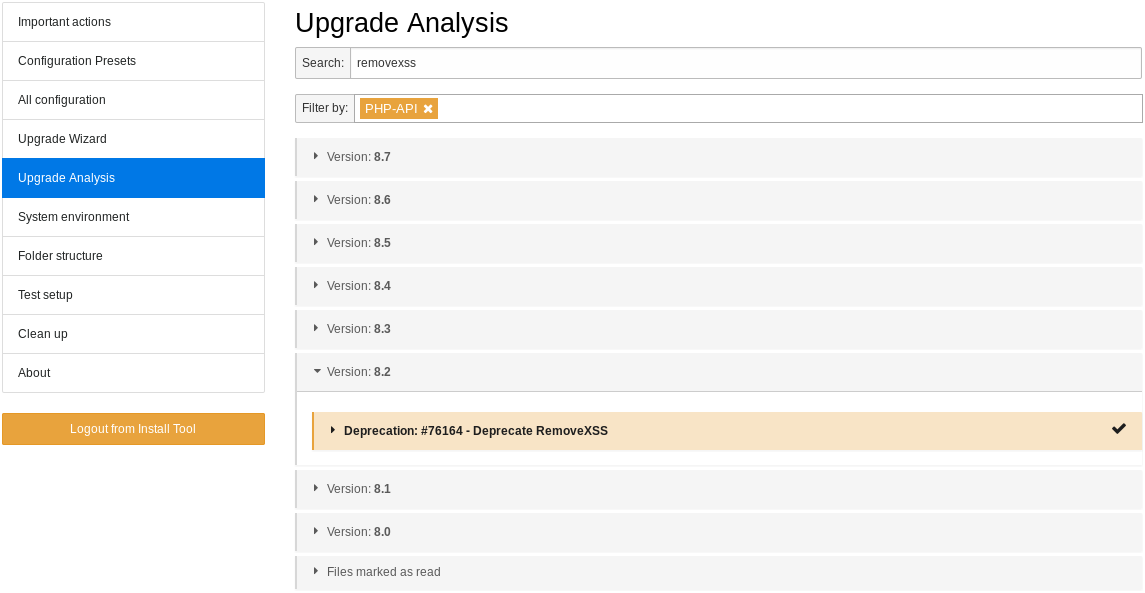
\includegraphics[width=0.45\linewidth]{BackendUserInterface/install-tool-upgrade-analysis.png}
	\end{figure}

\end{frame}

% ------------------------------------------------------------------------------
% LTXE-SLIDE-START
% LTXE-SLIDE-UID:		917ce622-d4a3e46d-100779d5-a8cab15a
% LTXE-SLIDE-ORIGIN:	9702aaf4-f02bbc35-67902b2e-42855506 English
% LTXE-SLIDE-TITLE:		Install Tool: Upgrade Analysis
% LTXE-SLIDE-REFERENCE:	#78222: Dump Class Loading Information UI in Install Tool
% ------------------------------------------------------------------------------

\begin{frame}[fragile]
	\frametitle{Backend User Interface}
	\framesubtitle{Install Tool: Dump Autoload Information}

	In order to re-generate class loading information, a new action has been added
	to the Install Tool to dump autoload information.

	\begin{figure}
		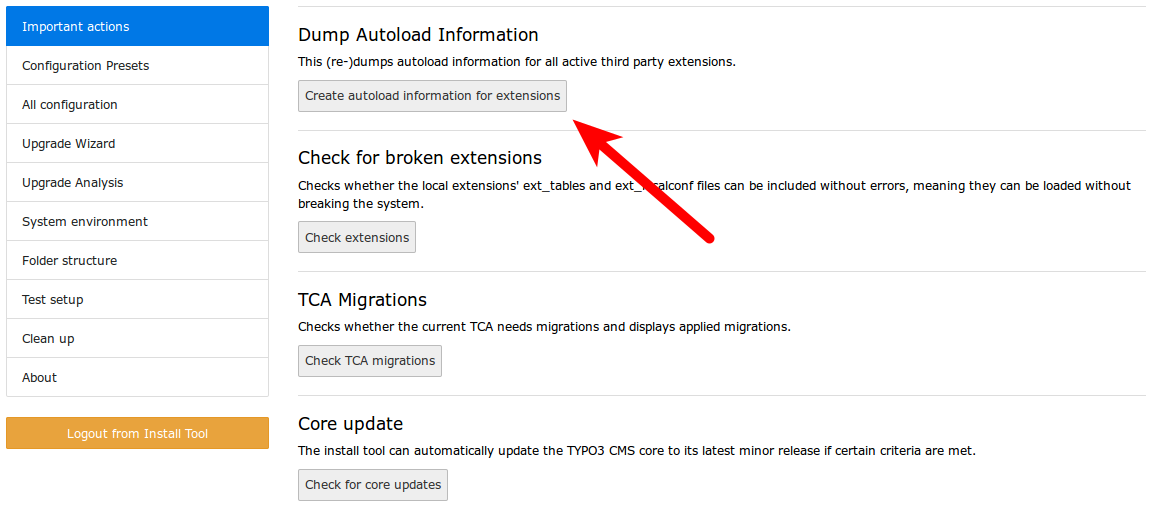
\includegraphics[width=0.8\linewidth]{BackendUserInterface/78222.png}
	\end{figure}

\end{frame}

% ------------------------------------------------------------------------------
% LTXE-SLIDE-START
% LTXE-SLIDE-UID:		aa93fe3c-cdb0c1a5-d021c6d0-e3a3c0f9
% LTXE-SLIDE-ORIGIN:	5a194e82-8eac7f1b-ef2730da-61d781b2 English
% LTXE-SLIDE-TITLE:		Install Tool: TCA Migration Messages
% LTXE-SLIDE-REFERENCE:	#77799: Display TCA migration messages in Install Tool
% ------------------------------------------------------------------------------

\begin{frame}[fragile]
	\frametitle{Backend User Interface}
	\framesubtitle{Install Tool: TCA Migration Messages}

	TCA migration message(s) can be checked/listed in the Install Tool now.

	\begin{figure}
		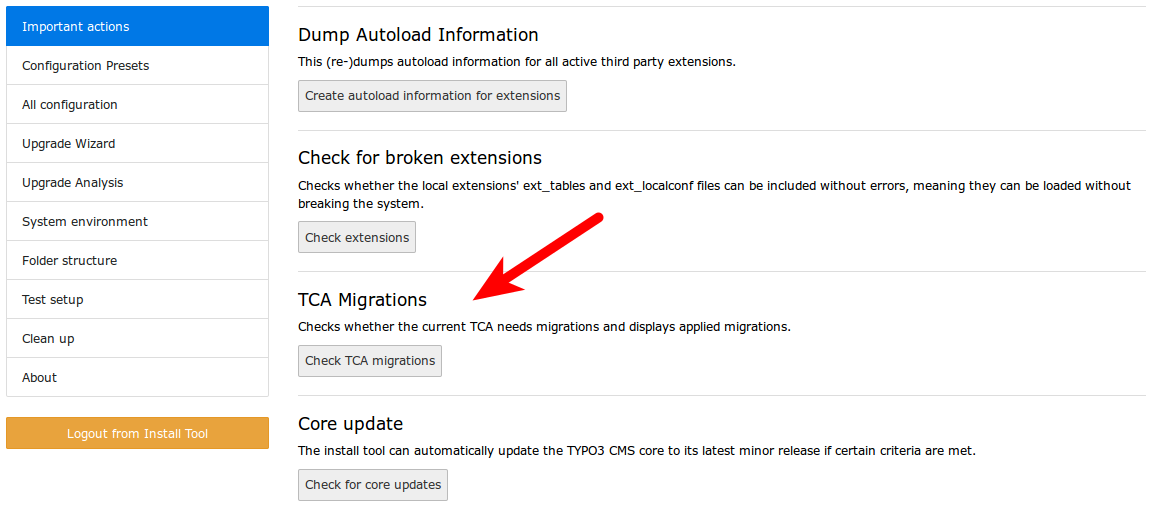
\includegraphics[width=0.8\linewidth]{BackendUserInterface/77799.png}
	\end{figure}

\end{frame}

% ------------------------------------------------------------------------------
% LTXE-SLIDE-START
% LTXE-SLIDE-UID:		419f61a2-e1da07ec-1d7c0209-cc1e889e
% LTXE-SLIDE-ORIGIN:	1e11eae3-872938ec-9612c092-444c408a English
% LTXE-SLIDE-TITLE:		sys_language records are sortable now
% LTXE-SLIDE-REFERENCE:	#77652: Make sys_language records sortable
% ------------------------------------------------------------------------------

\begin{frame}[fragile]
	\frametitle{In-Depth Changes}
	\framesubtitle{\texttt{sys\_language} Records}

	To improve usability, \texttt{sys\_language} records are sortable now.

	\begin{figure}
		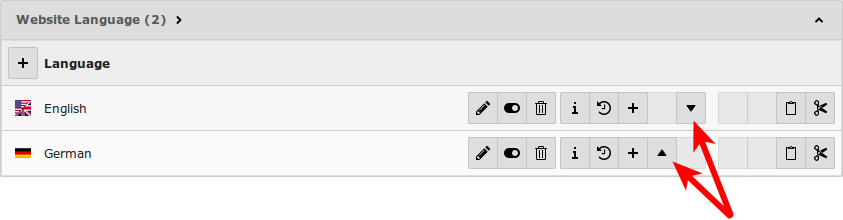
\includegraphics[width=0.8\linewidth]{BackendUserInterface/77652.png}
	\end{figure}

\end{frame}

% ------------------------------------------------------------------------------
% LTXE-SLIDE-START
% LTXE-SLIDE-UID:		c8e67bd3-e4204c3f-231d2a36-3bd04096
% LTXE-SLIDE-ORIGIN:	a82823ff-94b9520f-5e6d6056-95f1a797 English
% LTXE-SLIDE-TITLE:		#77668: Hide table listing below group element
% ------------------------------------------------------------------------------

\begin{frame}[fragile]
	\frametitle{TSconfig \& TypoScript}
	\framesubtitle{Table Listing Below Group Element}

	\begin{itemize}

		\item The TCA configuration option \texttt{disable\_controls} of type "group"
			has a new setting \texttt{allowedTables} now, which hides the hint about
			allowed tables to be referenced in the group field.

	\end{itemize}

	\begin{figure}
		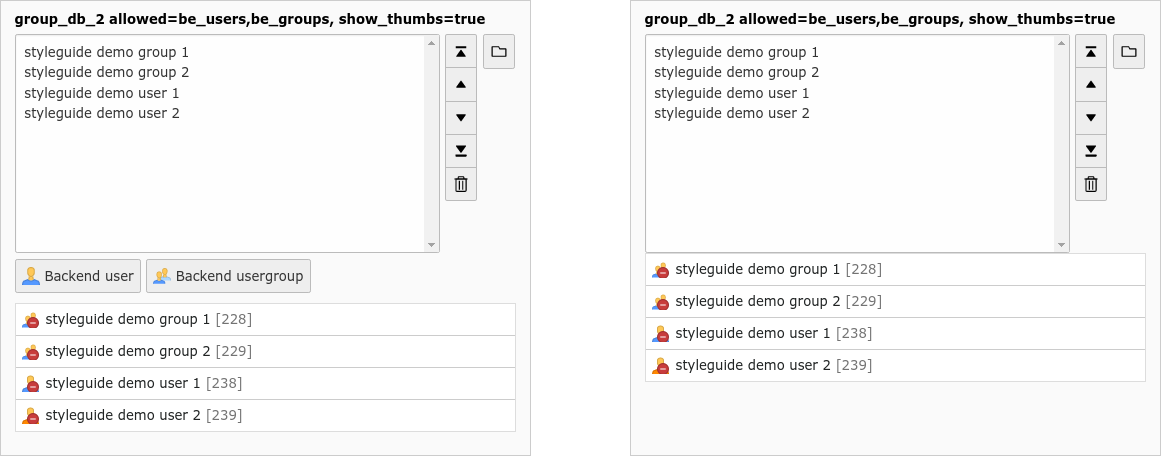
\includegraphics[width=0.85\linewidth]{BackendUserInterface/77668.png}
	\end{figure}

\end{frame}

% ------------------------------------------------------------------------------
